% Created by tikzDevice version 0.12.3 on 2019-12-11 20:53:34
% !TEX encoding = UTF-8 Unicode
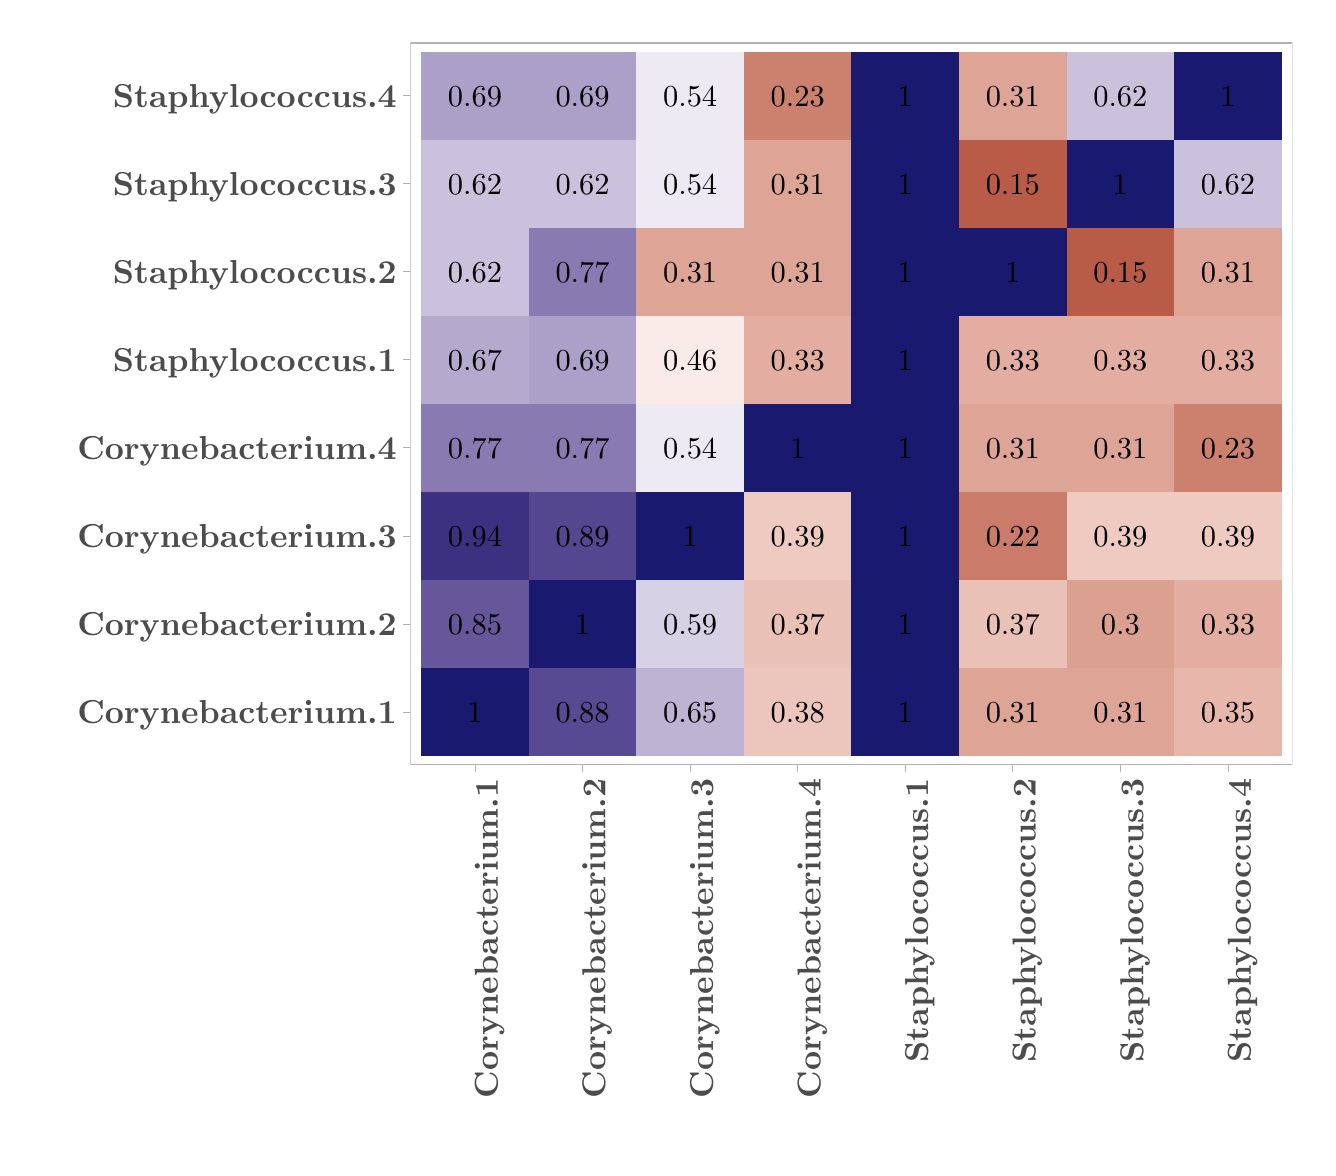
\begin{tikzpicture}[x=1pt,y=1pt]
\definecolor{fillColor}{RGB}{255,255,255}
\path[use as bounding box,fill=fillColor,fill opacity=0.00] (0,0) rectangle (462.53,404.71);
\begin{scope}
\path[clip] (  0.00,  0.00) rectangle (462.53,404.71);
\definecolor{drawColor}{RGB}{255,255,255}
\definecolor{fillColor}{RGB}{255,255,255}

\path[draw=drawColor,line width= 0.6pt,line join=round,line cap=round,fill=fillColor] (  0.00,  0.00) rectangle (462.53,404.71);
\end{scope}
\begin{scope}
\path[clip] (138.33,138.33) rectangle (457.03,399.21);
\definecolor{fillColor}{RGB}{255,255,255}

\path[fill=fillColor] (138.33,138.33) rectangle (457.03,399.21);
\definecolor{fillColor}{RGB}{25,25,112}

\path[fill=fillColor] (142.21,141.51) rectangle (181.08,173.32);
\definecolor{fillColor}{RGB}{88,74,146}

\path[fill=fillColor] (181.08,141.51) rectangle (219.95,173.32);
\definecolor{fillColor}{RGB}{189,179,211}

\path[fill=fillColor] (219.95,141.51) rectangle (258.81,173.32);
\definecolor{fillColor}{RGB}{236,198,188}

\path[fill=fillColor] (258.81,141.51) rectangle (297.68,173.32);
\definecolor{fillColor}{RGB}{25,25,112}

\path[fill=fillColor] (297.68,141.51) rectangle (336.54,173.32);
\definecolor{fillColor}{RGB}{222,165,151}

\path[fill=fillColor] (336.54,141.51) rectangle (375.41,173.32);

\path[fill=fillColor] (375.41,141.51) rectangle (414.28,173.32);
\definecolor{fillColor}{RGB}{231,183,172}

\path[fill=fillColor] (414.28,141.51) rectangle (453.14,173.32);
\definecolor{fillColor}{RGB}{102,87,154}

\path[fill=fillColor] (142.21,173.32) rectangle (181.08,205.14);
\definecolor{fillColor}{RGB}{25,25,112}

\path[fill=fillColor] (181.08,173.32) rectangle (219.95,205.14);
\definecolor{fillColor}{RGB}{215,209,229}

\path[fill=fillColor] (219.95,173.32) rectangle (258.81,205.14);
\definecolor{fillColor}{RGB}{234,193,183}

\path[fill=fillColor] (258.81,173.32) rectangle (297.68,205.14);
\definecolor{fillColor}{RGB}{25,25,112}

\path[fill=fillColor] (297.68,173.32) rectangle (336.54,205.14);
\definecolor{fillColor}{RGB}{234,193,183}

\path[fill=fillColor] (336.54,173.32) rectangle (375.41,205.14);
\definecolor{fillColor}{RGB}{220,160,145}

\path[fill=fillColor] (375.41,173.32) rectangle (414.28,205.14);
\definecolor{fillColor}{RGB}{227,174,161}

\path[fill=fillColor] (414.28,173.32) rectangle (453.14,205.14);
\definecolor{fillColor}{RGB}{60,49,129}

\path[fill=fillColor] (142.21,205.14) rectangle (181.08,236.95);
\definecolor{fillColor}{RGB}{84,70,143}

\path[fill=fillColor] (181.08,205.14) rectangle (219.95,236.95);
\definecolor{fillColor}{RGB}{25,25,112}

\path[fill=fillColor] (219.95,205.14) rectangle (258.81,236.95);
\definecolor{fillColor}{RGB}{238,202,193}

\path[fill=fillColor] (258.81,205.14) rectangle (297.68,236.95);
\definecolor{fillColor}{RGB}{25,25,112}

\path[fill=fillColor] (297.68,205.14) rectangle (336.54,236.95);
\definecolor{fillColor}{RGB}{202,123,105}

\path[fill=fillColor] (336.54,205.14) rectangle (375.41,236.95);
\definecolor{fillColor}{RGB}{238,202,193}

\path[fill=fillColor] (375.41,205.14) rectangle (414.28,236.95);

\path[fill=fillColor] (414.28,205.14) rectangle (453.14,236.95);
\definecolor{fillColor}{RGB}{137,123,177}

\path[fill=fillColor] (142.21,236.95) rectangle (181.08,268.77);

\path[fill=fillColor] (181.08,236.95) rectangle (219.95,268.77);
\definecolor{fillColor}{RGB}{237,234,243}

\path[fill=fillColor] (219.95,236.95) rectangle (258.81,268.77);
\definecolor{fillColor}{RGB}{25,25,112}

\path[fill=fillColor] (258.81,236.95) rectangle (297.68,268.77);

\path[fill=fillColor] (297.68,236.95) rectangle (336.54,268.77);
\definecolor{fillColor}{RGB}{222,165,151}

\path[fill=fillColor] (336.54,236.95) rectangle (375.41,268.77);

\path[fill=fillColor] (375.41,236.95) rectangle (414.28,268.77);
\definecolor{fillColor}{RGB}{204,128,110}

\path[fill=fillColor] (414.28,236.95) rectangle (453.14,268.77);
\definecolor{fillColor}{RGB}{180,170,206}

\path[fill=fillColor] (142.21,268.77) rectangle (181.08,300.58);
\definecolor{fillColor}{RGB}{171,160,200}

\path[fill=fillColor] (181.08,268.77) rectangle (219.95,300.58);
\definecolor{fillColor}{RGB}{249,236,232}

\path[fill=fillColor] (219.95,268.77) rectangle (258.81,300.58);
\definecolor{fillColor}{RGB}{227,174,161}

\path[fill=fillColor] (258.81,268.77) rectangle (297.68,300.58);
\definecolor{fillColor}{RGB}{25,25,112}

\path[fill=fillColor] (297.68,268.77) rectangle (336.54,300.58);
\definecolor{fillColor}{RGB}{227,174,161}

\path[fill=fillColor] (336.54,268.77) rectangle (375.41,300.58);

\path[fill=fillColor] (375.41,268.77) rectangle (414.28,300.58);

\path[fill=fillColor] (414.28,268.77) rectangle (453.14,300.58);
\definecolor{fillColor}{RGB}{202,194,220}

\path[fill=fillColor] (142.21,300.58) rectangle (181.08,332.40);
\definecolor{fillColor}{RGB}{137,123,177}

\path[fill=fillColor] (181.08,300.58) rectangle (219.95,332.40);
\definecolor{fillColor}{RGB}{222,165,151}

\path[fill=fillColor] (219.95,300.58) rectangle (258.81,332.40);

\path[fill=fillColor] (258.81,300.58) rectangle (297.68,332.40);
\definecolor{fillColor}{RGB}{25,25,112}

\path[fill=fillColor] (297.68,300.58) rectangle (336.54,332.40);

\path[fill=fillColor] (336.54,300.58) rectangle (375.41,332.40);
\definecolor{fillColor}{RGB}{184,91,71}

\path[fill=fillColor] (375.41,300.58) rectangle (414.28,332.40);
\definecolor{fillColor}{RGB}{222,165,151}

\path[fill=fillColor] (414.28,300.58) rectangle (453.14,332.40);
\definecolor{fillColor}{RGB}{202,194,220}

\path[fill=fillColor] (142.21,332.40) rectangle (181.08,364.22);

\path[fill=fillColor] (181.08,332.40) rectangle (219.95,364.22);
\definecolor{fillColor}{RGB}{237,234,243}

\path[fill=fillColor] (219.95,332.40) rectangle (258.81,364.22);
\definecolor{fillColor}{RGB}{222,165,151}

\path[fill=fillColor] (258.81,332.40) rectangle (297.68,364.22);
\definecolor{fillColor}{RGB}{25,25,112}

\path[fill=fillColor] (297.68,332.40) rectangle (336.54,364.22);
\definecolor{fillColor}{RGB}{184,91,71}

\path[fill=fillColor] (336.54,332.40) rectangle (375.41,364.22);
\definecolor{fillColor}{RGB}{25,25,112}

\path[fill=fillColor] (375.41,332.40) rectangle (414.28,364.22);
\definecolor{fillColor}{RGB}{202,194,220}

\path[fill=fillColor] (414.28,332.40) rectangle (453.14,364.22);
\definecolor{fillColor}{RGB}{171,160,200}

\path[fill=fillColor] (142.21,364.22) rectangle (181.08,396.03);

\path[fill=fillColor] (181.08,364.22) rectangle (219.95,396.03);
\definecolor{fillColor}{RGB}{237,234,243}

\path[fill=fillColor] (219.95,364.22) rectangle (258.81,396.03);
\definecolor{fillColor}{RGB}{204,128,110}

\path[fill=fillColor] (258.81,364.22) rectangle (297.68,396.03);
\definecolor{fillColor}{RGB}{25,25,112}

\path[fill=fillColor] (297.68,364.22) rectangle (336.54,396.03);
\definecolor{fillColor}{RGB}{222,165,151}

\path[fill=fillColor] (336.54,364.22) rectangle (375.41,396.03);
\definecolor{fillColor}{RGB}{202,194,220}

\path[fill=fillColor] (375.41,364.22) rectangle (414.28,396.03);
\definecolor{fillColor}{RGB}{25,25,112}

\path[fill=fillColor] (414.28,364.22) rectangle (453.14,396.03);
\definecolor{drawColor}{RGB}{0,0,0}

\node[text=drawColor,anchor=base,inner sep=0pt, outer sep=0pt, scale=  1.10] at (161.65,153.61) {1};

\node[text=drawColor,anchor=base,inner sep=0pt, outer sep=0pt, scale=  1.10] at (200.51,153.61) {0.88};

\node[text=drawColor,anchor=base,inner sep=0pt, outer sep=0pt, scale=  1.10] at (239.38,153.61) {0.65};

\node[text=drawColor,anchor=base,inner sep=0pt, outer sep=0pt, scale=  1.10] at (278.24,153.61) {0.38};

\node[text=drawColor,anchor=base,inner sep=0pt, outer sep=0pt, scale=  1.10] at (317.11,153.61) {1};

\node[text=drawColor,anchor=base,inner sep=0pt, outer sep=0pt, scale=  1.10] at (355.98,153.61) {0.31};

\node[text=drawColor,anchor=base,inner sep=0pt, outer sep=0pt, scale=  1.10] at (394.84,153.61) {0.31};

\node[text=drawColor,anchor=base,inner sep=0pt, outer sep=0pt, scale=  1.10] at (433.71,153.61) {0.35};

\node[text=drawColor,anchor=base,inner sep=0pt, outer sep=0pt, scale=  1.10] at (161.65,185.43) {0.85};

\node[text=drawColor,anchor=base,inner sep=0pt, outer sep=0pt, scale=  1.10] at (200.51,185.43) {1};

\node[text=drawColor,anchor=base,inner sep=0pt, outer sep=0pt, scale=  1.10] at (239.38,185.43) {0.59};

\node[text=drawColor,anchor=base,inner sep=0pt, outer sep=0pt, scale=  1.10] at (278.24,185.43) {0.37};

\node[text=drawColor,anchor=base,inner sep=0pt, outer sep=0pt, scale=  1.10] at (317.11,185.43) {1};

\node[text=drawColor,anchor=base,inner sep=0pt, outer sep=0pt, scale=  1.10] at (355.98,185.43) {0.37};

\node[text=drawColor,anchor=base,inner sep=0pt, outer sep=0pt, scale=  1.10] at (394.84,185.43) {0.3};

\node[text=drawColor,anchor=base,inner sep=0pt, outer sep=0pt, scale=  1.10] at (433.71,185.43) {0.33};

\node[text=drawColor,anchor=base,inner sep=0pt, outer sep=0pt, scale=  1.10] at (161.65,217.25) {0.94};

\node[text=drawColor,anchor=base,inner sep=0pt, outer sep=0pt, scale=  1.10] at (200.51,217.25) {0.89};

\node[text=drawColor,anchor=base,inner sep=0pt, outer sep=0pt, scale=  1.10] at (239.38,217.25) {1};

\node[text=drawColor,anchor=base,inner sep=0pt, outer sep=0pt, scale=  1.10] at (278.24,217.25) {0.39};

\node[text=drawColor,anchor=base,inner sep=0pt, outer sep=0pt, scale=  1.10] at (317.11,217.25) {1};

\node[text=drawColor,anchor=base,inner sep=0pt, outer sep=0pt, scale=  1.10] at (355.98,217.25) {0.22};

\node[text=drawColor,anchor=base,inner sep=0pt, outer sep=0pt, scale=  1.10] at (394.84,217.25) {0.39};

\node[text=drawColor,anchor=base,inner sep=0pt, outer sep=0pt, scale=  1.10] at (433.71,217.25) {0.39};

\node[text=drawColor,anchor=base,inner sep=0pt, outer sep=0pt, scale=  1.10] at (161.65,249.06) {0.77};

\node[text=drawColor,anchor=base,inner sep=0pt, outer sep=0pt, scale=  1.10] at (200.51,249.06) {0.77};

\node[text=drawColor,anchor=base,inner sep=0pt, outer sep=0pt, scale=  1.10] at (239.38,249.06) {0.54};

\node[text=drawColor,anchor=base,inner sep=0pt, outer sep=0pt, scale=  1.10] at (278.24,249.06) {1};

\node[text=drawColor,anchor=base,inner sep=0pt, outer sep=0pt, scale=  1.10] at (317.11,249.06) {1};

\node[text=drawColor,anchor=base,inner sep=0pt, outer sep=0pt, scale=  1.10] at (355.98,249.06) {0.31};

\node[text=drawColor,anchor=base,inner sep=0pt, outer sep=0pt, scale=  1.10] at (394.84,249.06) {0.31};

\node[text=drawColor,anchor=base,inner sep=0pt, outer sep=0pt, scale=  1.10] at (433.71,249.06) {0.23};

\node[text=drawColor,anchor=base,inner sep=0pt, outer sep=0pt, scale=  1.10] at (161.65,280.88) {0.67};

\node[text=drawColor,anchor=base,inner sep=0pt, outer sep=0pt, scale=  1.10] at (200.51,280.88) {0.69};

\node[text=drawColor,anchor=base,inner sep=0pt, outer sep=0pt, scale=  1.10] at (239.38,280.88) {0.46};

\node[text=drawColor,anchor=base,inner sep=0pt, outer sep=0pt, scale=  1.10] at (278.24,280.88) {0.33};

\node[text=drawColor,anchor=base,inner sep=0pt, outer sep=0pt, scale=  1.10] at (317.11,280.88) {1};

\node[text=drawColor,anchor=base,inner sep=0pt, outer sep=0pt, scale=  1.10] at (355.98,280.88) {0.33};

\node[text=drawColor,anchor=base,inner sep=0pt, outer sep=0pt, scale=  1.10] at (394.84,280.88) {0.33};

\node[text=drawColor,anchor=base,inner sep=0pt, outer sep=0pt, scale=  1.10] at (433.71,280.88) {0.33};

\node[text=drawColor,anchor=base,inner sep=0pt, outer sep=0pt, scale=  1.10] at (161.65,312.69) {0.62};

\node[text=drawColor,anchor=base,inner sep=0pt, outer sep=0pt, scale=  1.10] at (200.51,312.69) {0.77};

\node[text=drawColor,anchor=base,inner sep=0pt, outer sep=0pt, scale=  1.10] at (239.38,312.69) {0.31};

\node[text=drawColor,anchor=base,inner sep=0pt, outer sep=0pt, scale=  1.10] at (278.24,312.69) {0.31};

\node[text=drawColor,anchor=base,inner sep=0pt, outer sep=0pt, scale=  1.10] at (317.11,312.69) {1};

\node[text=drawColor,anchor=base,inner sep=0pt, outer sep=0pt, scale=  1.10] at (355.98,312.69) {1};

\node[text=drawColor,anchor=base,inner sep=0pt, outer sep=0pt, scale=  1.10] at (394.84,312.69) {0.15};

\node[text=drawColor,anchor=base,inner sep=0pt, outer sep=0pt, scale=  1.10] at (433.71,312.69) {0.31};

\node[text=drawColor,anchor=base,inner sep=0pt, outer sep=0pt, scale=  1.10] at (161.65,344.51) {0.62};

\node[text=drawColor,anchor=base,inner sep=0pt, outer sep=0pt, scale=  1.10] at (200.51,344.51) {0.62};

\node[text=drawColor,anchor=base,inner sep=0pt, outer sep=0pt, scale=  1.10] at (239.38,344.51) {0.54};

\node[text=drawColor,anchor=base,inner sep=0pt, outer sep=0pt, scale=  1.10] at (278.24,344.51) {0.31};

\node[text=drawColor,anchor=base,inner sep=0pt, outer sep=0pt, scale=  1.10] at (317.11,344.51) {1};

\node[text=drawColor,anchor=base,inner sep=0pt, outer sep=0pt, scale=  1.10] at (355.98,344.51) {0.15};

\node[text=drawColor,anchor=base,inner sep=0pt, outer sep=0pt, scale=  1.10] at (394.84,344.51) {1};

\node[text=drawColor,anchor=base,inner sep=0pt, outer sep=0pt, scale=  1.10] at (433.71,344.51) {0.62};

\node[text=drawColor,anchor=base,inner sep=0pt, outer sep=0pt, scale=  1.10] at (161.65,376.32) {0.69};

\node[text=drawColor,anchor=base,inner sep=0pt, outer sep=0pt, scale=  1.10] at (200.51,376.32) {0.69};

\node[text=drawColor,anchor=base,inner sep=0pt, outer sep=0pt, scale=  1.10] at (239.38,376.32) {0.54};

\node[text=drawColor,anchor=base,inner sep=0pt, outer sep=0pt, scale=  1.10] at (278.24,376.32) {0.23};

\node[text=drawColor,anchor=base,inner sep=0pt, outer sep=0pt, scale=  1.10] at (317.11,376.32) {1};

\node[text=drawColor,anchor=base,inner sep=0pt, outer sep=0pt, scale=  1.10] at (355.98,376.32) {0.31};

\node[text=drawColor,anchor=base,inner sep=0pt, outer sep=0pt, scale=  1.10] at (394.84,376.32) {0.62};

\node[text=drawColor,anchor=base,inner sep=0pt, outer sep=0pt, scale=  1.10] at (433.71,376.32) {1};
\definecolor{drawColor}{gray}{0.70}

\path[draw=drawColor,line width= 0.6pt,line join=round,line cap=round] (138.33,138.33) rectangle (457.03,399.21);
\end{scope}
\begin{scope}
\path[clip] (  0.00,  0.00) rectangle (462.53,404.71);
\definecolor{drawColor}{gray}{0.30}

\node[text=drawColor,anchor=base east,inner sep=0pt, outer sep=0pt, scale=  1.20] at (133.38,153.28) {\bfseries Corynebacterium.1};

\node[text=drawColor,anchor=base east,inner sep=0pt, outer sep=0pt, scale=  1.20] at (133.38,185.09) {\bfseries Corynebacterium.2};

\node[text=drawColor,anchor=base east,inner sep=0pt, outer sep=0pt, scale=  1.20] at (133.38,216.91) {\bfseries Corynebacterium.3};

\node[text=drawColor,anchor=base east,inner sep=0pt, outer sep=0pt, scale=  1.20] at (133.38,248.72) {\bfseries Corynebacterium.4};

\node[text=drawColor,anchor=base east,inner sep=0pt, outer sep=0pt, scale=  1.20] at (133.38,280.54) {\bfseries Staphylococcus.1};

\node[text=drawColor,anchor=base east,inner sep=0pt, outer sep=0pt, scale=  1.20] at (133.38,312.35) {\bfseries Staphylococcus.2};

\node[text=drawColor,anchor=base east,inner sep=0pt, outer sep=0pt, scale=  1.20] at (133.38,344.17) {\bfseries Staphylococcus.3};

\node[text=drawColor,anchor=base east,inner sep=0pt, outer sep=0pt, scale=  1.20] at (133.38,375.98) {\bfseries Staphylococcus.4};
\end{scope}
\begin{scope}
\path[clip] (  0.00,  0.00) rectangle (462.53,404.71);
\definecolor{drawColor}{gray}{0.70}

\path[draw=drawColor,line width= 0.3pt,line join=round] (135.58,157.42) --
	(138.33,157.42);

\path[draw=drawColor,line width= 0.3pt,line join=round] (135.58,189.23) --
	(138.33,189.23);

\path[draw=drawColor,line width= 0.3pt,line join=round] (135.58,221.05) --
	(138.33,221.05);

\path[draw=drawColor,line width= 0.3pt,line join=round] (135.58,252.86) --
	(138.33,252.86);

\path[draw=drawColor,line width= 0.3pt,line join=round] (135.58,284.68) --
	(138.33,284.68);

\path[draw=drawColor,line width= 0.3pt,line join=round] (135.58,316.49) --
	(138.33,316.49);

\path[draw=drawColor,line width= 0.3pt,line join=round] (135.58,348.31) --
	(138.33,348.31);

\path[draw=drawColor,line width= 0.3pt,line join=round] (135.58,380.12) --
	(138.33,380.12);
\end{scope}
\begin{scope}
\path[clip] (  0.00,  0.00) rectangle (462.53,404.71);
\definecolor{drawColor}{gray}{0.70}

\path[draw=drawColor,line width= 0.3pt,line join=round] (161.65,135.58) --
	(161.65,138.33);

\path[draw=drawColor,line width= 0.3pt,line join=round] (200.51,135.58) --
	(200.51,138.33);

\path[draw=drawColor,line width= 0.3pt,line join=round] (239.38,135.58) --
	(239.38,138.33);

\path[draw=drawColor,line width= 0.3pt,line join=round] (278.24,135.58) --
	(278.24,138.33);

\path[draw=drawColor,line width= 0.3pt,line join=round] (317.11,135.58) --
	(317.11,138.33);

\path[draw=drawColor,line width= 0.3pt,line join=round] (355.98,135.58) --
	(355.98,138.33);

\path[draw=drawColor,line width= 0.3pt,line join=round] (394.84,135.58) --
	(394.84,138.33);

\path[draw=drawColor,line width= 0.3pt,line join=round] (433.71,135.58) --
	(433.71,138.33);
\end{scope}
\begin{scope}
\path[clip] (  0.00,  0.00) rectangle (462.53,404.71);
\definecolor{drawColor}{gray}{0.30}

\node[text=drawColor,rotate= 90.00,anchor=base east,inner sep=0pt, outer sep=0pt, scale=  1.20] at (169.93,133.38) {\bfseries Corynebacterium.1};

\node[text=drawColor,rotate= 90.00,anchor=base east,inner sep=0pt, outer sep=0pt, scale=  1.20] at (208.79,133.38) {\bfseries Corynebacterium.2};

\node[text=drawColor,rotate= 90.00,anchor=base east,inner sep=0pt, outer sep=0pt, scale=  1.20] at (247.66,133.38) {\bfseries Corynebacterium.3};

\node[text=drawColor,rotate= 90.00,anchor=base east,inner sep=0pt, outer sep=0pt, scale=  1.20] at (286.53,133.38) {\bfseries Corynebacterium.4};

\node[text=drawColor,rotate= 90.00,anchor=base east,inner sep=0pt, outer sep=0pt, scale=  1.20] at (325.39,133.38) {\bfseries Staphylococcus.1};

\node[text=drawColor,rotate= 90.00,anchor=base east,inner sep=0pt, outer sep=0pt, scale=  1.20] at (364.26,133.38) {\bfseries Staphylococcus.2};

\node[text=drawColor,rotate= 90.00,anchor=base east,inner sep=0pt, outer sep=0pt, scale=  1.20] at (403.12,133.38) {\bfseries Staphylococcus.3};

\node[text=drawColor,rotate= 90.00,anchor=base east,inner sep=0pt, outer sep=0pt, scale=  1.20] at (441.99,133.38) {\bfseries Staphylococcus.4};
\end{scope}
\end{tikzpicture}
